\documentclass[11pt,landscape]{article}
\usepackage{multicol}
\usepackage{calc}
\usepackage{ifthen}
\usepackage[landscape]{geometry}
\usepackage{hyperref}
\usepackage{amsmath}
\usepackage{graphicx}
\usepackage{float}

% To make this come out properly in landscape mode, do one of the following
% 1.
%  pdflatex latexsheet.tex
%
% 2.
%  latex latexsheet.tex
%  dvips -P pdf  -t landscape latexsheet.dvi
%  ps2pdf latexsheet.ps


% If you're reading this, be prepared for confusion.  Making this was
% a learning experience for me, and it shows.  Much of the placement
% was hacked in; if you make it better, let me know...


% 2008-04
% Changed page margin code to use the geometry package. Also added code for
% conditional page margins, depending on paper size. Thanks to Uwe Ziegenhagen
% for the suggestions.

% 2006-08
% Made changes based on suggestions from Gene Cooperman. <gene at ccs.neu.edu>


% To Do:
% \listoffigures \listoftables
% \setcounter{secnumdepth}{0}


% This sets page margins to .5 inch if using letter paper, and to 1cm
% if using A4 paper. (This probably isn't strictly necessary.)
% If using another size paper, use default 1cm margins.
\ifthenelse{\lengthtest { \paperwidth = 11in}}
	{ \geometry{top=.5in,left=.5in,right=.5in,bottom=.5in} }
	{\ifthenelse{ \lengthtest{ \paperwidth = 297mm}}
		{\geometry{top=1cm,left=1cm,right=1cm,bottom=1cm} }
		{\geometry{top=1cm,left=1cm,right=1cm,bottom=1cm} }
	}

% Turn off header and footer
\pagestyle{empty}
 

% Redefine section commands to use less space
\makeatletter
\renewcommand{\section}{\@startsection{section}{1}{0mm}%
                                {-1ex plus -.5ex minus -.2ex}%
                                {0.5ex plus .2ex}%x
                                {\normalfont\large\bfseries}}
\renewcommand{\subsection}{\@startsection{subsection}{2}{0mm}%
                                {-1explus -.5ex minus -.2ex}%
                                {0.5ex plus .2ex}%
                                {\normalfont\normalsize\bfseries}}
\renewcommand{\subsubsection}{\@startsection{subsubsection}{3}{0mm}%
                                {-1ex plus -.5ex minus -.2ex}%
                                {1ex plus .2ex}%
                                {\normalfont\small\bfseries}}
\makeatother

% Define BibTeX command
\def\BibTeX{{\rm B\kern-.05em{\sc i\kern-.025em b}\kern-.08em
    T\kern-.1667em\lower.7ex\hbox{E}\kern-.125emX}}

% Don't print section numbers
\setcounter{secnumdepth}{0}


\setlength{\parindent}{0pt}
\setlength{\parskip}{0pt plus 0.5ex}


% -----------------------------------------------------------------------

\begin{document}

\raggedright
\footnotesize
\begin{multicols}{3}


% multicol parameters
% These lengths are set only within the two main columns
%\setlength{\columnseprule}{0.25pt}
\setlength{\premulticols}{1pt}
\setlength{\postmulticols}{1pt}
\setlength{\multicolsep}{1pt}
\setlength{\columnsep}{2pt}

\begin{center}
     \Large{\textbf{EECS 230 Cheat Sheet}} \\
\end{center}

\section{Constants}
\begin{tabular}{@{}ll@{}}
$q$              & $1.6 \times 10^{-19}$ C\\
$\varepsilon_0$  & $8.854 \times 10^{-12}$ F/m\\
$\mu_0$          & $4\pi\times 10^{-7}$ H/m \\
$u_p$ & $\frac{c}{\sqrt{\varepsilon_r}}$ \\
\end{tabular}

\section{Identities}
$e^{jx} + e^{-jx} = 2cosx$ \\
$e^{jx} - e^{-jx} = 2sinx$ \\
$\hat{\textbf{x}}\times\hat{\textbf{y}} = \hat{\textbf{z}}, 
\hat{\textbf{y}}\times\hat{\textbf{z}} = \hat{\textbf{x}},
\hat{\textbf{z}}\times\hat{\textbf{x}} = \hat{\textbf{y}}$ \\
$\textbf{A}\times\textbf{B} = \hat{\textbf{n}}ABsin\theta_{AB}$ \\
$\textbf{A}\cdot\textbf{B} = ABcos\theta_{AB}$ \\
\section{Transients}
\newlength{\MyLen}
\settowidth{\MyLen}{\texttt{letterpaper}/\texttt{a4paper} \ }
At t = 0, the source cannot only see $Z_0$ of the transmission line and not the load. Thus, $I_1^+ = \frac{V_g}{R_g + Z_0}$ and $V_1^+ = I_1^+Z_0$. $\Gamma_L = \frac{R_L-Z_0}{R_L+Z_0}$ and $\Gamma_g = \frac{R_g - Z_0}{R_g+Z_0}$. Thus, $V_1^- = \Gamma_LV_1^+$ and $I_1^- = -\Gamma_LI_1^+$. $V_\infty = \frac{V_gR_L}{R_g+R_L}$ and $I_\infty = \frac{V_\infty}{R_L}$


\section{Electrostatics}
\settowidth{\MyLen}{\texttt{multicol} }
$y(x,t) = Ae^{-\alpha x}cos(\omega t - \beta x + \phi_0)$ \\
$u_p = \frac{\lambda}{T} = f\lambda = \frac{\omega}{\beta}$ \\

If the signs of $\omega t$ and $\beta x$ are the same, the wave is traveling in the negative x-direction, else the positive x-direction. \\
$y(x,t) = Ae^{-\alpha x}e^{j(\beta x + \phi_0)}$ \\


\section{Transmission Line Equations}
$-\dfrac{d\tilde{V}(z)}{dz} = (R' + j\omega L')\tilde{I}(z)$ \\
$-\dfrac{d\tilde{I}(z)}{dz} = (G' + j\omega C')\tilde{V}(z)$ \\
$ \tilde{V}(z) = V_0^+ e^{-\gamma z} + V_0^- e^{\gamma z} $ \\
$ \tilde{I}(z) = I_0^+ e^{-\gamma z} + I_0^- e^{\gamma z} $ \\
$ Z_0 = \frac{V_0^+}{I_0^+} = \frac{-V_0^-}{I_0^-} $ \\
$Z_0 = \sqrt{\dfrac{R' + j\omega L'}{G' + j\omega C'}}$ \\
$\gamma = \alpha + j\beta = \sqrt{(R'+j\omega L')(G' + j\omega C')}$ \\
$\vert\tilde{V}(z)\vert = \vert V_0^+ \vert\sqrt{[e^{-2\alpha z} + \vert\Gamma\vert^2e^{2\alpha z} + 2\vert\Gamma\vert cos(2\beta z + \varphi_{\Gamma})]}$
$\vert\tilde{V}\vert_{max} = \vert V_0^+ \vert (1+\vert\Gamma\vert)$, $\vert\tilde{V}\vert_{min} = \vert V_0^+ \vert (1-\vert\Gamma\vert)$


\subsection{Lossless Line}
$\alpha = 0$, $\beta = \omega\sqrt{L'C'} $ \\
$ Z_0 = \sqrt{\frac{L'}{C'}} $ \\
$ \Gamma = \dfrac{Z_L - Z_0}{Z_L + Z_0} = \dfrac{z_L - 1}{z_L + 1} = \dfrac{I_0^-}{I_0^+} = -\dfrac{V_0^-}{V_0^+}$ \\
$ S = \dfrac{1 + \vert\Gamma\vert}{1 - \vert\Gamma\vert}$


\subsection{Wave Impedance}
$Z_{in} = Z_0\left(\dfrac{1 + \Gamma e^{j\beta l}}{1 - \Gamma e^{j\beta l}}\right)$ \\
$Z_{in} = Z_0\left(\dfrac{z_L + jtan\beta l}{1 + jz_Ltan\beta l}\right)$ \\
$V_0^+ = \left(\dfrac{\tilde{V}_gZ_{in}}{Z_g + Z_{in}}\right)\left(\dfrac{1}{e^{j\beta l}+ \Gamma e^{-j\beta l}}\right)$ \\
$v(d, t) = \Re[\tilde{V}(d)e^{j\omega t}]$


\subsection{Special Cases}
$Z_{in}^{sc} = jZ_0 tan\beta l$ \\
$Z_{in}^{oc} = -jZ_0 cot\beta l$ \\
$Z_0 = \sqrt{Z_{in}^{sc}Z_{in}^{oc}}$ \\
$tan\beta l = \sqrt{-\dfrac{Z_{in}^{sc}}{Z_{in}^{oc}}}$ \\
$Z_{in} = \dfrac{Z_0^2}{Z_L}$ for quarter-wavelength transformers

\subsection{Power}
$P_{av}^i = \dfrac{\vert V_0^+ \vert^2}{2Z_0}$ Average Power from the initial wave \\
$P_{av}^r = -\vert\Gamma\vert^2P_{av}^i$ Average Power from the reflected wave \\
$P_{av} = P_{av}^i + P_{av}^r$ \\
$P_{av} = \frac{1}{2}\vert\tilde{I}_L\vert^2R_L = \frac{1}{2}\Re(V_{in}I^*_{in})$
%---------------------------------------------------------------------------

\end{multicols}

\begin{multicols}{2}
\setlength{\premulticols}{1pt}
\setlength{\postmulticols}{1pt}
\setlength{\multicolsep}{1pt}
\setlength{\columnsep}{2pt}
\begin{figure}[H]
    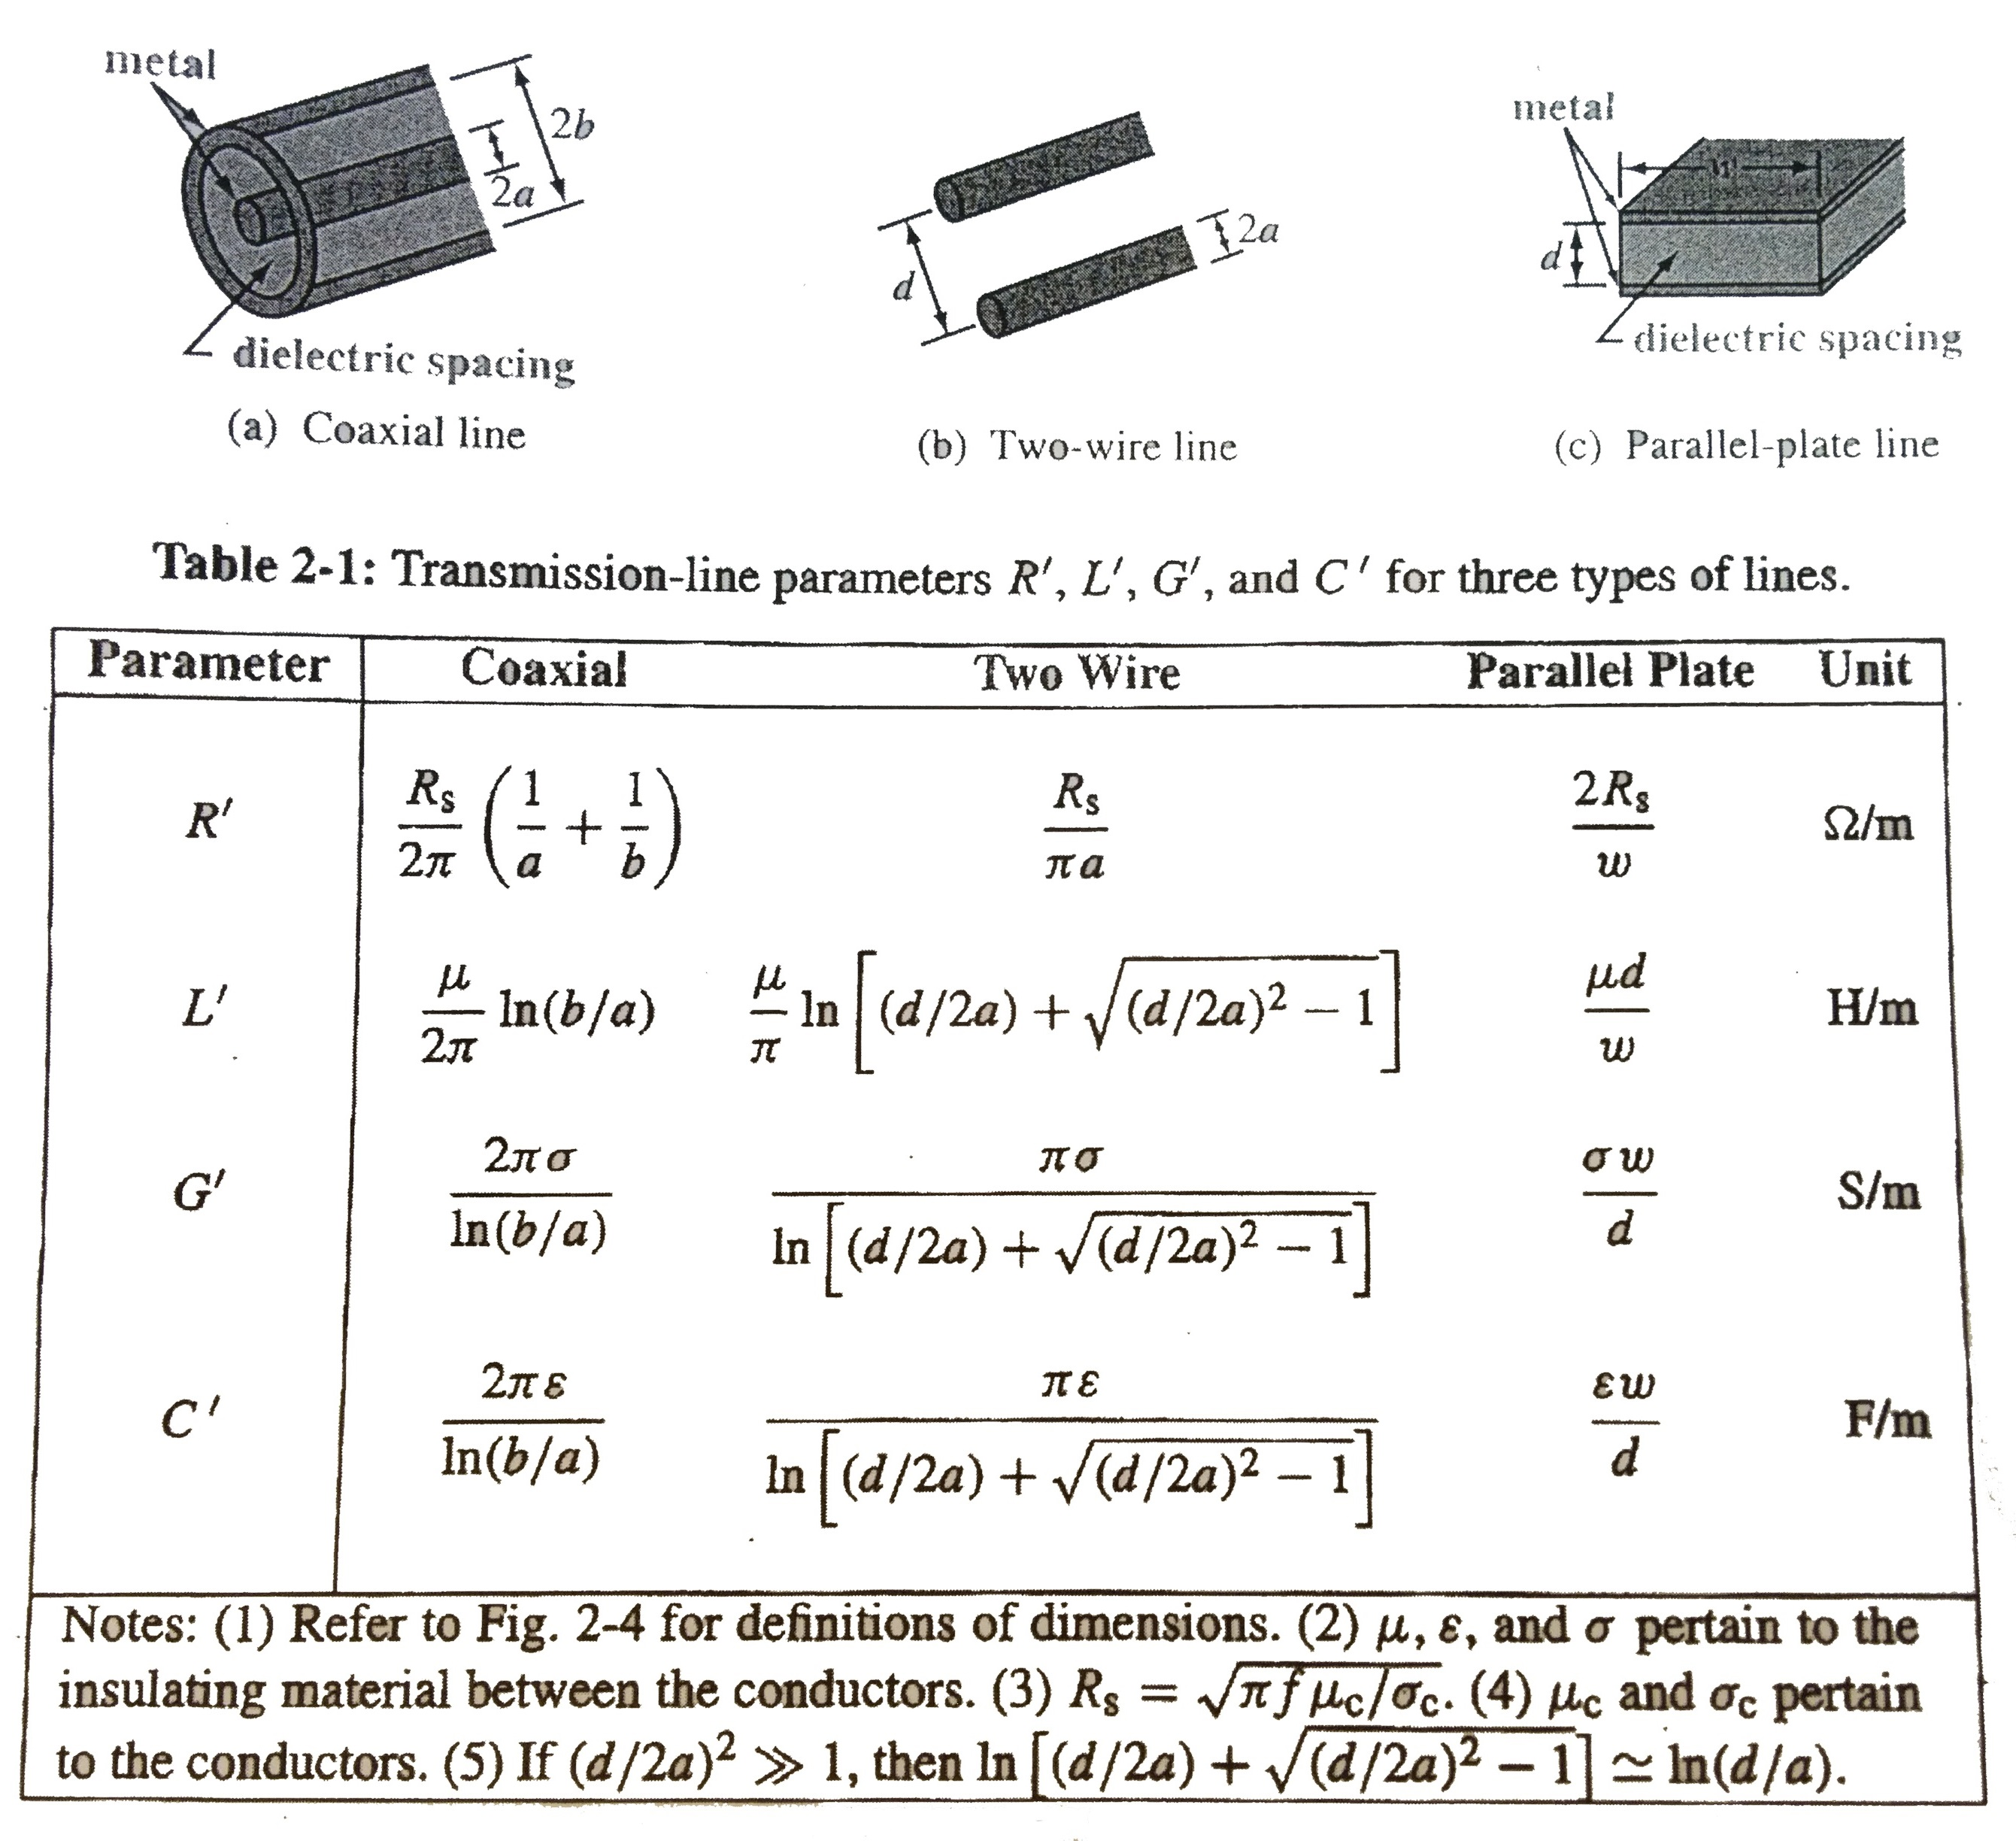
\includegraphics[scale=0.13]{./Images/1/TLtypes.jpg}
\end{figure}
\begin{figure}[H]
    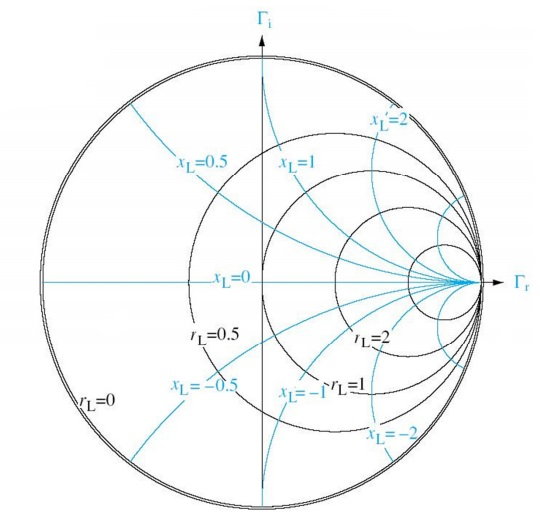
\includegraphics[scale=0.7]{./Images/1/smithchart.jpg}
\end{figure}
\end{multicols}

\end{document}